% Compile twice with pdfLaTeX. No cover page is included.
% Times-equivalent font, 12 pt body and 1.5 line spacing are explicit below.
\documentclass[12pt,a4paper]{article}
\usepackage[margin=0.9in]{geometry}
% Times-compatible text and mathematics; no machine-specific font fallback.
\usepackage[T1]{fontenc}
\usepackage{mathptmx}
\usepackage{courier}
\usepackage{amsmath,amssymb,graphicx,booktabs,array,setspace,titlesec,caption}
\usepackage[hidelinks]{hyperref}
\usepackage{float}
\usepackage[table]{xcolor}
\usepackage{fancyhdr}
\definecolor{Navy}{HTML}{15334F}
\pagestyle{fancy}
\fancyhf{}
\fancyfoot[R]{\fontsize{10}{12}\selectfont\color{Navy}\thepage}
\renewcommand{\headrulewidth}{0pt}
\setlength{\headheight}{23pt}
\addtolength{\topmargin}{-9pt}
\arrayrulecolor{black}
\setcounter{secnumdepth}{0}
\setcounter{tocdepth}{2}
\onehalfspacing
\setlength{\parindent}{0pt}
\setlength{\parskip}{3pt}
\setlength{\emergencystretch}{1em}
\setlength{\abovedisplayskip}{7pt}
\setlength{\belowdisplayskip}{7pt}
\titleformat{\section}{\fontsize{15}{18}\selectfont\bfseries\color{Navy}}{}{0pt}{}
\titleformat{\subsection}{\fontsize{12}{15}\selectfont\bfseries\color{Navy}}{}{0pt}{}
\titlespacing*{\section}{0pt}{9pt}{5pt}
\titlespacing*{\subsection}{0pt}{5pt}{2pt}
\captionsetup{font=normalsize,labelfont={bf,color=Navy},justification=centering,singlelinecheck=false,skip=5pt}
\graphicspath{{figures/}}
\hypersetup{pdftitle={Room Occupancy Estimation Using a Naive Bayes Classifier},pdfauthor={}}
\begin{document}
\pagenumbering{roman}
\tableofcontents
\clearpage
\pagenumbering{arabic}

\begin{center}
{\fontsize{18}{22}\selectfont\bfseries\color{Navy} Room Occupancy Estimation Using a\par Na\"ive Bayes Classifier}\par
\vspace{6pt}
{\fontsize{10}{12}\selectfont\textbf{Repository:} \url{https://github.com/md-abdullah-al-ahad/room-occupancy-naive-bayes}}\par
\end{center}

\section{Chapter 1: Background Study}
Room occupancy estimation classifies how many people occupy a room from environmental measurements. This assignment implements Na\"ive Bayes from scratch for zero to three occupants, then examines transfer between days and the information available from individual sensor groups.

\subsection{1.1 Bayes' theorem}
Bayes' theorem updates a class belief after observing evidence~\cite[Sec.~2.2.3]{murphy}:
\begin{equation}
P(c\mid\mathbf{x})=\frac{P(\mathbf{x}\mid c)P(c)}{P(\mathbf{x})}.
\end{equation}
The \textbf{prior}, $P(c)$, is the class probability before observing the sensors. The \textbf{likelihood}, $P(\mathbf{x}\mid c)$, describes the measurements given the class. The \textbf{evidence}, $P(\mathbf{x})$, normalizes the result, while the \textbf{posterior}, $P(c\mid\mathbf{x})$, is the updated class probability. For example, a high CO$_2$ reading may increase the probability of occupancy relative to the prior. For continuous measurements, the likelihood and evidence are probability densities.

\subsection{1.2 Derivation and the independence assumption}
Before simplification, the likelihood is the \emph{joint} conditional distribution of all features: $P(\mathbf{x}\mid c)=P(x_1,\ldots,x_d\mid c)$. Learning every feature interaction is difficult. Na\"ive Bayes instead assumes conditional independence~\cite[Sec.~3.5]{murphy}:
\begin{equation}
P(x_1,\ldots,x_d\mid c)\approx\prod_{j=1}^{d}P(x_j\mid c),\qquad
\hat c=\underset{c}{\arg\max}\left[\log P(c)+\sum_{j=1}^{d}\log P(x_j\mid c)\right].
\label{eq:decision}
\end{equation}
For a fixed reading $\mathbf{x}$, the evidence $P(\mathbf{x})$ is identical for every candidate class; dividing by it cannot change which score is largest. It is therefore omitted for classification, but normalization is needed for posterior probabilities. Logarithms prevent underflow when multiplying small likelihoods.

The assumption can fail when nearby light sensors remain correlated even after fixing occupancy. In text, ``credit'' and ``card'' may co-occur within spam messages, so their occurrences are also dependent. Nevertheless, a classifier needs the correct \emph{ordering} of class scores, not perfectly estimated probabilities. Fewer parameters also reduce estimation demands; useful predictions can therefore remain possible despite imperfect assumptions, although confidence may be unreliable.

\clearpage
\subsection{1.3 Applications}
\textbf{Spam detection.} Word occurrences and message attributes provide evidence for spam versus legitimate mail. Learning their class-specific frequencies supports rapid filtering, while smoothing handles words rarely observed in training.

\textbf{Sentiment analysis.} A text classifier uses words such as ``excellent'' or ``disappointing'' to distinguish positive and negative reviews. Simple word-based models may miss negation, such as ``not excellent'', because word relationships are simplified.

\textbf{Disease prediction.} Symptoms and test results can update the probability of a disease relative to its prior prevalence. Correlated symptoms may violate independence; predictions require appropriate validation and do not replace clinical judgement.

\section{Chapter 2: Dataset Selection and Preparation}
\subsection{2.1 Source and observations}
The UCI Room Occupancy Estimation dataset~\cite{dataset} contains measurements and manually recorded occupancy labels from one controlled room. The unchanged CSV is distributed under CC BY 4.0. There are \textbf{10,129 rows}, 16 sensor predictors and date/time.

The target, \texttt{Room\_Occupancy\_Count}, records zero to three people.

The predictors are four temperatures, four light readings, four sound readings, CO$_2$ level and slope, and two binary PIR motion readings. Class counts are 8,228 (81.23\%), 459 (4.53\%), 748 (7.38\%) and 694 (6.85\%) for classes 0--3, respectively.

\subsection{2.2 Checks, preprocessing and splitting}
There are no missing or non-finite sensor values, duplicate complete rows or duplicate timestamps. Binary PIR values need no encoding. Standardization is unnecessary because continuous features have separate likelihood parameters. Date/time is excluded from predictors and retained for temporal evaluation.

A stratified random 80/20 split uses seed 42. Rounding each class's test count upward yields \textbf{8,102 training} and \textbf{2,027 test} readings; all model parameters use training data only. Although UCI describes four collection days, the CSV covers seven calendar dates between 22 December 2017 and 11 January 2018, with gaps. Only 22 and 23 December contain all classes. These days support the transfer experiment; a chronological 80/20 split lacks class 1 in testing.

\clearpage
\section{Chapter 3: Model Building and Implementation}
\subsection{3.1 Likelihoods and training}
The classifier combines Gaussian likelihoods for 14 continuous measurements with Bernoulli likelihoods for two PIR features. For class $c$ with $n_c$ training rows, the prior is $\pi_c=n_c/n$. Continuous-feature parameters are
\begin{equation}
\mu_{cj}=\frac{1}{n_c}\sum_{i:y_i=c}x_{ij},\qquad
v_{cj}=\frac{1}{n_c}\sum_{i:y_i=c}(x_{ij}-\mu_{cj})^2.
\end{equation}
The Gaussian density is
\begin{equation}
p(x_j\mid c)=\frac{1}{\sqrt{2\pi v_{cj}}}
\exp\!\left[-\frac{(x_j-\mu_{cj})^2}{2v_{cj}}\right].
\end{equation}
To avoid zero variances, $v_{cj}$ is floored at $10^{-6}\max(V_j,10^{-12})$, where $V_j$ is feature $j$'s variance across training readings. For binary feature $b$, Laplace smoothing gives
\begin{equation}
q_{cb}=\frac{\sum_{i:y_i=c}x_{ib}+1}{n_c+2},\qquad
p(x_b\mid c)=q_{cb}^{x_b}(1-q_{cb})^{1-x_b}.
\end{equation}
Smoothing values are fixed in advance. No test-based hyperparameter tuning is performed.

\subsection{3.2 Prediction and implementation workflow}
For each test reading, the implementation adds the log prior and the Gaussian and Bernoulli log-likelihoods, then selects the highest-scoring class using Equation~\eqref{eq:decision}. Subtracting the largest score before exponentiation permits stable probability normalization when needed.

The \textbf{full commented implementation is in the submitted notebook}. pandas loads the data, NumPy implements splitting, training, prediction and metrics, and Matplotlib plots the results~\cite{numpy,pandas,matplotlib}. No scikit-learn functions are used.

\vspace{4pt}
\noindent\begin{minipage}{\linewidth}
\textbf{Training and prediction (pseudocode)}\\
\texttt{TRAIN:} For each class, estimate prior, means and variances.\\
\hspace*{1em}Floor variances and estimate smoothed PIR probabilities.\\
\texttt{PREDICT:} For each reading, calculate each class's log score.\\
\hspace*{1em}Add log prior and feature log-likelihoods; return the highest-scoring class.
\end{minipage}
\vspace{4pt}

Saved indices make splits traceable. Checks verify scores, probability normalization, disjoint partitions and confusion-matrix orientation.

\clearpage
\section{Chapter 4: Results and Discussion}
\subsection{4.1 Main evaluation}
Precision is $TP/(TP+FP)$, recall is $TP/(TP+FN)$ and F1 is $2PR/(P+R)$; zero denominators give zero. Accuracy is the correct-prediction fraction. Macro averages weight classes equally. Confusion-matrix rows are actual labels; columns are predictions.

The classifier achieved \textbf{95.26\% accuracy}, \textbf{87.10\% macro-precision}, \textbf{90.85\% macro-recall} and \textbf{88.82\% macro-F1}. Predicting the most common training class (empty) gave 81.20\% test accuracy and 22.41\% macro-F1, illustrating the imbalance problem.

\begin{table}[H]
\centering
\caption{Per-class performance on the 2,027 test readings.}
\begin{tabular}{rrrrr}
\toprule
\color{Navy}\bfseries Occupants & \color{Navy}\bfseries Precision (\%) & \color{Navy}\bfseries Recall (\%) & \color{Navy}\bfseries F1 (\%) & \color{Navy}\bfseries Support \\
\midrule
0 & 99.07 & 96.96 & 98.00 & 1,646 \\
1 & 100.00 & 97.83 & 98.90 & 92 \\
2 & 84.80 & 96.67 & 90.34 & 150 \\
3 & 64.52 & 71.94 & 68.03 & 139 \\
\bottomrule
\end{tabular}
\end{table}

\begin{figure}[H]
\centering
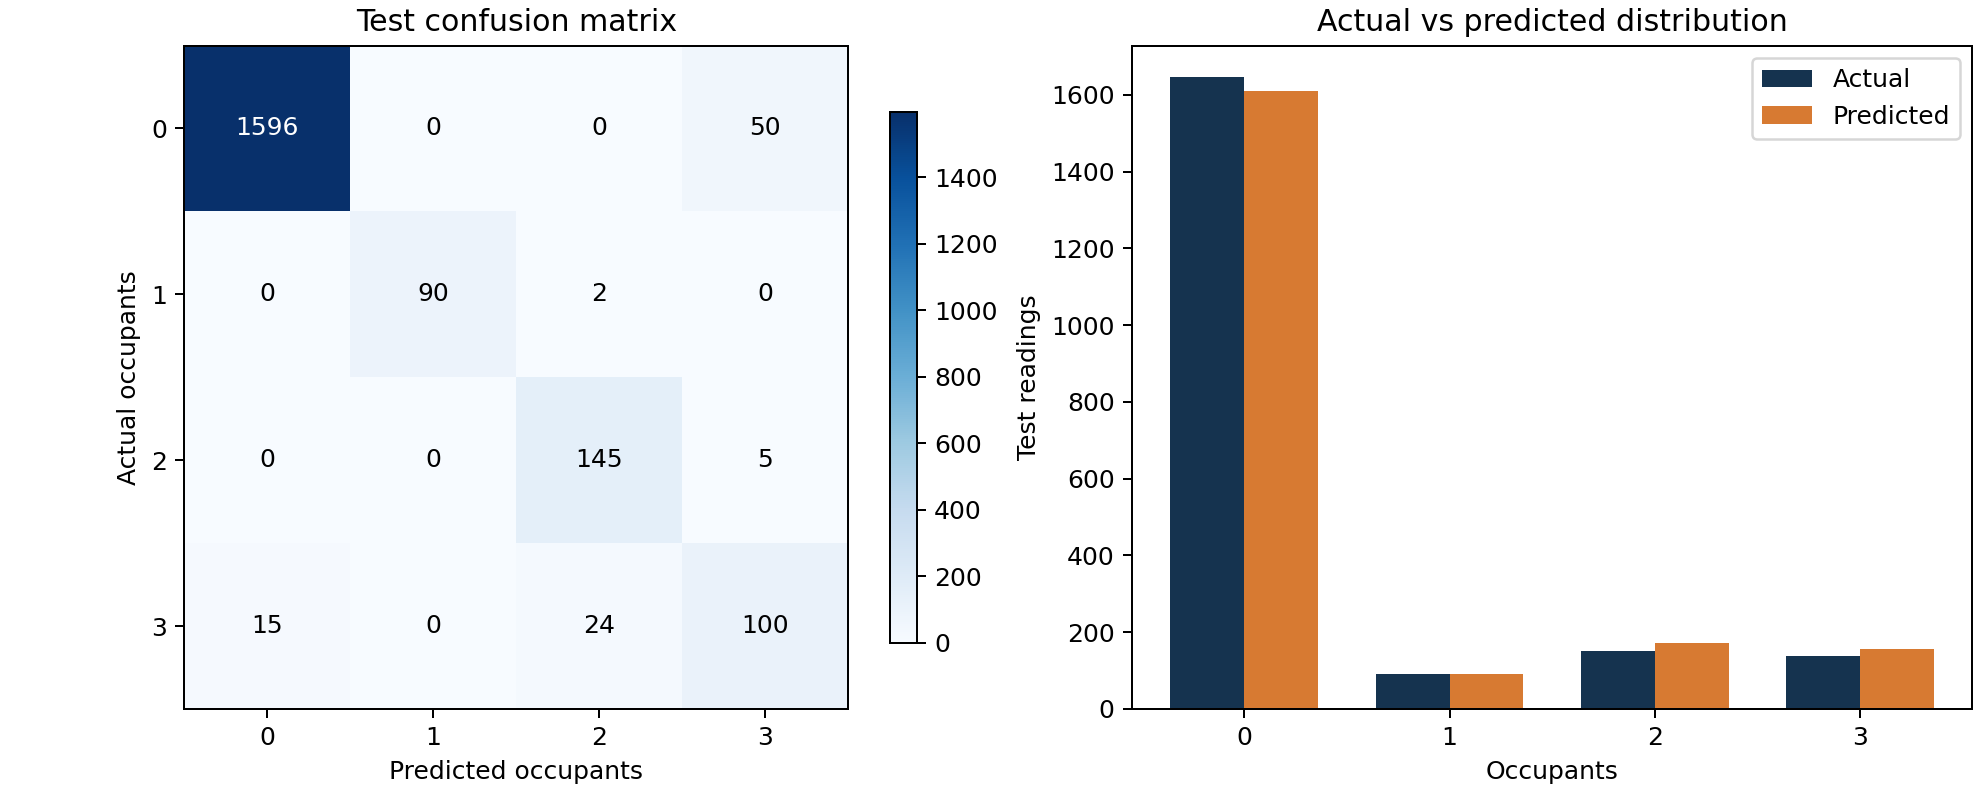
\includegraphics[width=0.86\linewidth]{main_evaluation.png}
\caption{Confusion matrix and actual versus predicted test-label counts.}
\end{figure}

Of 139 three-person readings, 100 were correct, 15 were labelled empty and 24 as two occupants. Fifty empty readings were labelled three occupants. Aggregate label counts therefore hide individual errors.

\subsection{4.2 Transfer between observed days}
Transfer uses 22 December (1,462 readings) and 23 December (2,779). Five random controls per direction pool the same days and match training/test class counts, using seeds 42--46.

Forward transfer achieved 99.21\% accuracy and 0.984 macro-F1; reverse transfer gave 70.04\% and 0.613. Matched random macro-F1 was $0.961\pm0.005$ forward and $0.968\pm0.007$ reverse (five-seed allocation SD). The asymmetry does not isolate causes; reverse transfer is not forecasting.

\clearpage
\subsection{4.3 Comparing sensor groups}
Predefined groups use identical main-split indices and fixed smoothing. Scores measure standalone performance, not unique contributions to the full model.

\begin{table}[H]
\centering
\caption{Sensor-group results on the same test readings.}
\begin{tabular}{lrrr}
\toprule
\color{Navy}\bfseries Sensor group & \color{Navy}\bfseries Inputs & \color{Navy}\bfseries Accuracy (\%) & \color{Navy}\bfseries Macro-F1 \\
\midrule
All sensors & 16 & 95.26 & 0.888 \\
Temperature only & 4 & 82.68 & 0.488 \\
Light only & 4 & 90.08 & 0.724 \\
Sound only & 4 & 88.16 & 0.551 \\
CO$_2$ level and slope & 2 & 84.95 & 0.509 \\
Motion only & 2 & 86.78 & 0.446 \\
\bottomrule
\end{tabular}
\end{table}
Light alone was strongest among individual groups, but three-person recall was only 12.23\%, versus 71.94\% with all sensors. High accuracy can therefore hide poor recognition of a specific count. This exploratory comparison does not establish hardware savings.

\section{Chapter 5: Conclusion}
The classifier achieved 95.26\% accuracy and 88.82\% macro-F1, exceeding the empty-room baseline. Weaker three-person performance, directional day transfer and sensor-group differences show why aggregate accuracy needs class-wise and contextual interpretation.

Evidence is limited to one controlled room with dependent readings. Gaussian and independence assumptions are approximate; CO$_2$ slope causality is unverified. Reused-test comparisons are exploratory and establish neither calibration, cross-room generalization nor deployment readiness. The contribution is transparent implementation and evaluation.

\vspace{4pt}
\begingroup
\onehalfspacing
\renewcommand{\refname}{References}
\phantomsection
\addcontentsline{toc}{section}{References}
\begin{thebibliography}{9}
\setlength{\itemsep}{2pt}
\setlength{\parskip}{0pt}
\bibitem{murphy} K. P. Murphy, \emph{Machine Learning: A Probabilistic Perspective}. Cambridge, MA: MIT Press, 2012, Secs.~2.2.3 and 3.5.
\bibitem{dataset} A. Singh and S. Chaudhari, ``Room Occupancy Estimation,'' UCI Machine Learning Repository, 2018. Dataset DOI: \url{https://doi.org/10.24432/C5P605}.
\bibitem{numpy} NumPy Developers, ``NumPy documentation.'' \url{https://numpy.org/doc/}. Implementation version: 2.3.5.
\bibitem{pandas} pandas Development Team, ``pandas documentation.'' \url{https://pandas.pydata.org/docs/}. Implementation version: 2.2.3.
\bibitem{matplotlib} Matplotlib Development Team, ``Matplotlib documentation.'' \url{https://matplotlib.org/stable/}.
\end{thebibliography}
\endgroup
\end{document}
